%\documentclass[3p]{elsarticle}
\documentclass[5p]{elsarticle}
\usepackage{natbib,graphicx,amsmath, mhchem,url,colortbl,fancyhdr,subfigure}
\usepackage{multicol}

\journal{EECS 551}

%\renewcommand{\headrulewidth}{0.4pt}
%\fancyhead[L]{}
%\fancyhead[R]{
%\includegraphics[width=4cm]{jpl.png}
%}
%\pagestyle{fancy}
%\date{}

\providecommand{\e}[1]{\ensuremath{\times 10^{#1}}}

%\begin{center}
%\includegraphics[width=0.15\textwidth]{./jpl.png}\\[1cm]
%\end{center}

\begin{document}
\begin{frontmatter}

\title{Blind Source Separation and Independent Component Analysis: A Review}
\author[jpl]{Jeremy Nash} %\corref{cor}}
\ead{nashj@umich.edu}
%\cortext[cor]{Corresponding author}

\author[jpl]{Ryan Garrone}
\ead{garrone@umich.edu}

\address[jpl]{Electrical Engineering Division, University of Michigan, Ann Arbor, MI 48109}

\begin{abstract}

Blind source separation (BSS) and independent component analysis (ICA) are generally based on a wide class of unsupervised learning algorithms and they found potential applications in many areas from engineering to neuroscience. A recent trend in BSS is to consider problems in the framework of matrix factorization or more general signals decomposition with probabilistic generative and tree structured graphical models and exploit a priori knowledge about true nature and structure of latent (hidden) variables or sources such as spatio-temporal decorrelation, statistical independence, sparseness, smoothness or lowest complexity in the sense e.g., of best predictability. The possible goal of such decomposition can be considered as the estimation of sources not necessary statistically independent and parameters of a mixing system or more generally as finding a new reduced or hierarchical and structured representation for the observed (sensor) data that can be interpreted as physically meaningful coding or blind source estimation. The key issue is to find a such transformation or coding (linear or nonlinear) which has true physical meaning and interpretation. We present a review of BSS and ICA, including various algorithms for static and dynamic models and their applications. The paper mainly consists of three parts: (1) BSS algorithms for static models (instantaneous mixtures); (2) extension of BSS and ICA incorporating with sparseness or non-negativity constraints; (3) BSS algorithms for dynamic models (convolutive mixtures).

\end{abstract}
\begin{keyword}
Independent Component Analysis \sep Blind Source Separation \sep information theory \sep feature extraction
\end{keyword}
\end{frontmatter}

%\newpage

\setcounter{topnumber}{1}
%\setcounter{tocdepth}{2}
%\tableofcontents

%\newpage

\begin{figure*}[t]
\begin{center}
\subfigure[]{
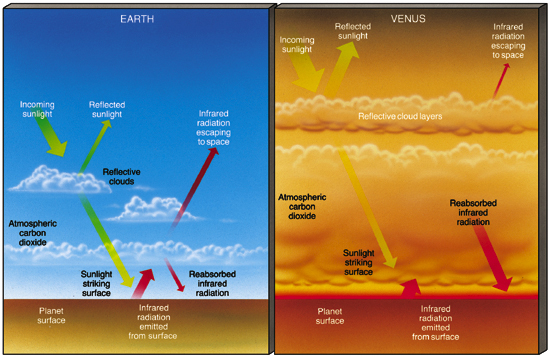
\includegraphics[scale=.35]{earth-venus.jpg}
\label{fig:awwnnprioriprof}
}
\subfigure[]{
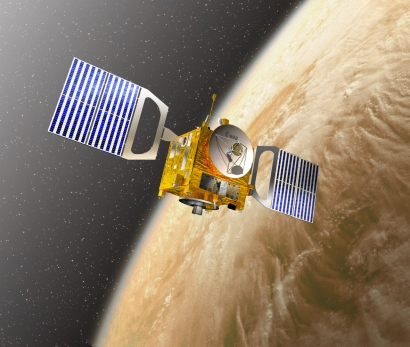
\includegraphics[scale=1.5]{venuscircle.jpg}
\label{fig:optdewwpth}
}
\end{center}
\caption{(a) Side-by-side comparison of Earth's and Venus' atmosphere; notice the thick layer of reflective clouds high above the surface of Venus. (b) An artist's depiction of the Venus Express satellite in orbit, carrying the VIRTIS-H Echelle spectrometer. }
\end{figure*}

\section{Introduction}
Lorem ipsum dolor sit amet, consectetur adipisicing elit, sed do eiusmod tempor incididunt ut labore et dolore magna aliqua. Ut enim ad minim veniam, quis nostrud exercitation ullamco laboris nisi ut aliquip ex ea commodo consequat. Duis aute irure dolor in reprehenderit in voluptate velit esse cillum dolore eu fugiat nulla pariatur. Excepteur sint occaecat cupidatat non proident, sunt in culpa qui officia deserunt mollit anim id est laborum.

\begin{enumerate}
\item First Item
\item Second Item
\item Third Item
\end{enumerate}

\section{Blind Source Separation Based on Spatio-Temporal Decorrelation and Non-Stationarity}

Lorem ipsum dolor sit amet, consectetur adipisicing elit, sed do eiusmod tempor incididunt ut labore et dolore magna aliqua. Ut enim ad minim veniam, quis nostrud exercitation ullamco laboris nisi ut aliquip ex ea commodo consequat. Duis aute irure dolor in reprehenderit in voluptate velit esse cillum dolore eu fugiat nulla pariatur. Excepteur sint occaecat cupidatat non proident, sunt in culpa qui officia deserunt mollit anim id est laborum.

\subsection{Subsection 1}

(1) Planetary Evolution: While Earth is an oasis for life, Venus developed into a hellish, inhospitable planet with a cloud deck of sulfuric acid and hurricane-speed winds. What caused the two planets to differ in evolution? Why did Venus lose all of its water?

(2) Climate Change on Earth: Atmospheric science addresses questions about the effects of gases and aerosols on our climate. What processes maintain the greenhouse effect and high temperatures on Venus? Why do the clouds on Venus rotate 60 times faster than the surface?

\subsection{Subsection 2}

Lorem ipsum dolor sit amet, consectetur adipisicing elit, sed do eiusmod tempor incididunt ut labore et dolore magna aliqua. Ut enim ad minim veniam, quis nostrud exercitation ullamco laboris nisi ut aliquip ex ea commodo consequat. Duis aute irure dolor in reprehenderit in voluptate velit esse cillum dolore eu fugiat nulla pariatur. Excepteur sint occaecat cupidatat non proident, sunt in culpa qui officia deserunt mollit anim id est laborum.

\begin{table}[b] \centering \caption{VIRTIS-H Spectral Orders}
  \begin{tabular}{|l|l|l|}
    \hline 
    \rowcolor[gray]{.7} Order & $\lambda$ min ($\mu$m) & $\lambda$ max ($\mu$m) \\ \hline
    Order 0 & 4.00342 & 4.98660 \\ \hline 
    Order 1 & 3.43527 & 4.28712 \\ \hline
    Order 2 & 3.00538 & 3.75714 \\ \hline
    Order 3 & 2.67117 & 3.34079 \\ \hline
    Order 4 & 2.40335 & 3.00673 \\ \hline
    Order 5 & 2.18426 & 2.73313 \\ \hline
    Order 6 & 2.00126 & 2.50554 \\ \hline
    Order 7 & 1.84486 & 2.31273 \\ \hline
  \end{tabular}
  \label{ordertable}
\end{table}


\section{Blind Source Extraction Using Linear Predictability and Adaptive Band-Pass Filters}

Lorem ipsum dolor sit amet, consectetur adipisicing elit, sed do eiusmod tempor incididunt ut labore et dolore magna aliqua. Ut enim ad minim veniam, quis nostrud exercitation ullamco laboris nisi ut aliquip ex ea commodo consequat. Duis aute irure dolor in reprehenderit in voluptate velit esse cillum dolore eu fugiat nulla pariatur. Excepteur sint occaecat cupidatat non proident, sunt in culpa qui officia deserunt mollit anim id est laborum.

\begin{description}
\item[Item 1] 

Lorem ipsum dolor sit amet, consectetur adipisicing elit, sed do eiusmod tempor incididunt ut labore et dolore magna aliqua. Ut enim ad minim veniam, quis nostrud exercitation ullamco laboris nisi ut aliquip ex ea commodo consequat. Duis aute irure dolor in reprehenderit in voluptate velit esse cillum dolore eu fugiat nulla pariatur. Excepteur sint occaecat cupidatat non proident, sunt in culpa qui officia deserunt mollit anim id est laborum.

\item[Item 2]

Lorem ipsum dolor sit amet, consectetur adipisicing elit, sed do eiusmod tempor incididunt ut labore et dolore magna aliqua. Ut enim ad minim veniam, quis nostrud exercitation ullamco laboris nisi ut aliquip ex ea commodo consequat. Duis aute irure dolor in reprehenderit in voluptate velit esse cillum dolore eu fugiat nulla pariatur. Excepteur sint occaecat cupidatat non proident, sunt in culpa qui officia deserunt mollit anim id est laborum.

\item[Item 3]

Lorem ipsum dolor sit amet, consectetur adipisicing elit, sed do eiusmod tempor incididunt ut labore et dolore magna aliqua. Ut enim ad minim veniam, quis nostrud exercitation ullamco laboris nisi ut aliquip ex ea commodo consequat. Duis aute irure dolor in reprehenderit in voluptate velit esse cillum dolore eu fugiat nulla pariatur. Excepteur sint occaecat cupidatat non proident, sunt in culpa qui officia deserunt mollit anim id est laborum.

\end{description}

\section{Independent Component Analysis}

Lorem ipsum dolor sit amet, consectetur adipisicing elit, sed do eiusmod tempor incididunt ut labore et dolore magna aliqua. Ut enim ad minim veniam, quis nostrud exercitation ullamco laboris nisi ut aliquip ex ea commodo consequat. Duis aute irure dolor in reprehenderit in voluptate velit esse cillum dolore eu fugiat nulla pariatur. Excepteur sint occaecat cupidatat non proident, sunt in culpa qui officia deserunt mollit anim id est laborum.

\section{Validity of ICA-based BSS Algorithms for Real-World Data} 

\subsection{Subsection}

Lorem ipsum dolor sit amet, consectetur adipisicing elit, sed do eiusmod tempor incididunt ut labore et dolore magna aliqua. Ut enim ad minim veniam, quis nostrud exercitation ullamco laboris nisi ut aliquip ex ea commodo consequat. Duis aute irure dolor in reprehenderit in voluptate velit esse cillum dolore eu fugiat nulla pariatur. Excepteur sint occaecat cupidatat non proide

We began with a broad survey of the current research on Venus atmospheric retrievals. Investigating the focus of other Venus research groups can be a useful guide for the choice of spectral windows, initial guess values, and atmospheric constituent selection in our experiments. The results of the survey show a strong interest in nightside retrievals of the 2.18 - 2.5 $\mu$m band (\citep{tsang2008tropospheric},\citep{tsang2010correlations},\citep{marcq2005latitudinal},\citep{tsang2009variability},\citep{marcq2008latitudinal}). There has also been some recent interest in daytime retrievals of the 4 - 5 $\mu$m band to characterize the non-LTE emissions of \ce{CO2} (\citep{peralta2010spatial},\citep{grassi2010thermal}).

\begin{figure*}[t]
\begin{center}
\subfigure[]{ 
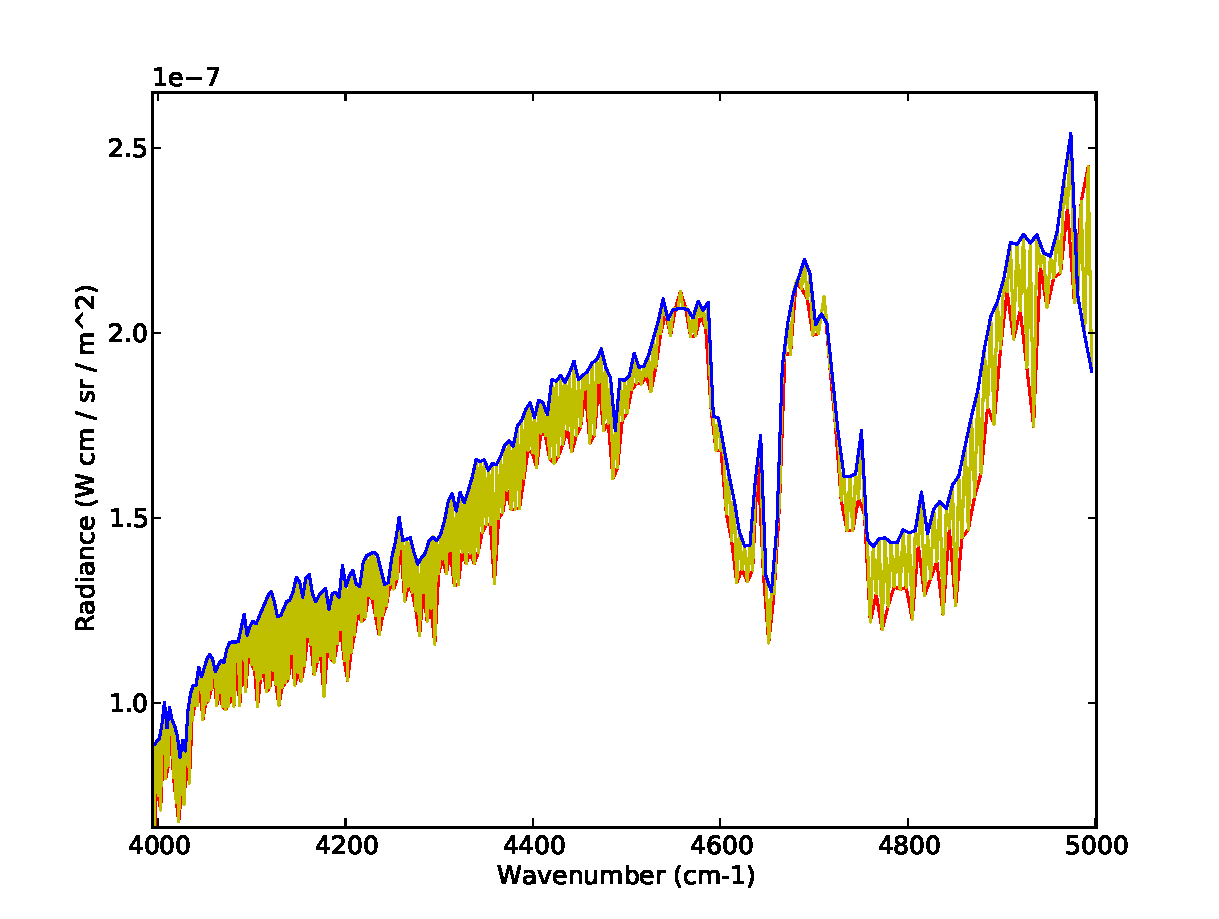
\includegraphics[scale=.4]{oddeveneffect.pdf}
\label{fig:oddeven}
}
\subfigure[]{ 
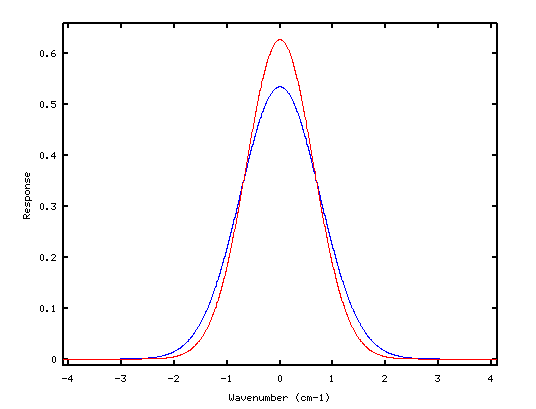
\includegraphics[scale=.40]{redlowwn_bluehighwn.png}
\label{fig:ils}
}
\end{center}
\caption{(a) The odd-even effect due to the imperfect flat-field of the detector matrix. The blue line represents the even pixel intensity values and the red line represents the odd pixel values.  (b) Theoretical Gaussian instrument line shapes. Red represents the ILS at the lowest pixel wavenumber in the sixth spectral order, while blue represents the highest wavenumber.}
\end{figure*}


While VIRTIS L1B products provide a one-to-one mapping between instrument pixels and wavelengths, we will adopt the ACOS method of describing spectral order dispersion with the polynomial $w = \alpha p^{2} + \beta p + \gamma$, where $w$ is wavenumber, $\alpha$ and $\beta$ represent wavelength resolution, $p$ is pixel number, and $\gamma$ is wavelength offset. The polynomial below describes the dispersion for the sixth spectral order.

\[
w = 2.6633\e{-3} p^{2} + 1.1301 p + 4001.2
\]

\noindent This form is mathematically convenient for the following reason: when we treat the polynomial coefficients as retrieval parameters, the retrieval adopts the semantics of solving for the lump effect of all Doppler shifts in the system. Thus, the dispersion polynomial provides a convenient way to account for the Doppler effects of unknown velocities; for VIRTIS-H retrievals, this allows us to sidestep unknowns in satellite velocity and Venus wind speed. 

\citet{cottini2011water} notes a pixel-dependent pattern noise called the ``odd-even'' effect, which is caused by the imperfect flat-field of the detector matrix. Her team chose to use only odd pixels for retrievals because it provided a better fit to their synthetic data. Figure~\ref{fig:oddeven} shows that the magnitude of the ``odd-even'' effect is comparable to the size of minor gas constituent signatures. Because we are skipping every other pixel and dropping the first nonphysical zero value, our dispersion polynomial for the sixth spectral order changes to the following:

\[
w = 0.010653 p^{2} + 2.2708 p + 4002.4
\]

\subsection{Venus ephemeris model}

ACOS uses a simple polynomial model based on day of year to calculate the Earth's distance from the sun. Since Venus's orbital period is 224.7 Earth days, we had to derive a new model that would be based both on Earth's year and day of year:

\[
d = .0049 \sin(2 \pi \frac{t + 21}{225}) + .72335
\]

\noindent where $d$ is solar distance in AU and $t$ is the number of days that have elapsed since April 11, 2006, 12PM, the day that Venus Express arrived at Venus.

\subsection{Wind model}

We use a simplified wind model based on \citet{sanchez2008variable} to describe the latitudinally dependent zonal windspeeds at the lower clouds (around 50 km). The zonal winds show a constant speed of -60$\pm$10 ms$^{-1}$ from the equator up to latitude $65^{\circ}$S and a steady decrease toward zero velocity at the poles.

\[
  v_{w}(\ell) = 
  \begin{cases} 
   -60 \text{ ms$^{-1}$} & \text{ for $\ell < 65^{\circ}$} \\ 
    1.96 |\ell| - 182.7 \text{ ms$^{-1}$}  & \text{ for $\ell \ge 65^{\circ}$ } 
  \end{cases}\\
\]

\noindent where $v_{w}$ is wind velocity and $\ell$ is latitude in degrees. The windspeeds above latitude $65^{\circ}$S were fit to figures from \citet{sanchez2008variable} using linear least squares.

ACOS currently only treats windspeed for Coxmunk surfaces. In this context, windspeed represents the speed at the surface of the ocean to model ocean churn for glint retrievals. 

\subsection{Index of refraction model}

The Rayleigh scattering cross-section is calculated using the following model from \citet{cox2001allen}:

\[
\sigma_{R} = \frac{24 \pi^{3}}{N_{s}^{2} \lambda^{4}} \frac{(n^{2} -1)^{2}}{(n^{2} + 2)^{2}} \frac{6 + 3 \rho}{6 - 7 \rho}
\]

\noindent where $\lambda$ is wavelength, $N_{s}$ is the number density of air at some pressure and temperature, $\rho$ is the depolarization factor, and $n_{s}$ is the index of refraction at the same pressure and temperature. According to Lorentz-Lorenz theory, the product of these two terms is invariant to pressure and temperature. 


\bibliographystyle{model1-num-names}
\bibliography{venus}
\end{document}
